% !TeX spellcheck = en_US

\section{Implementation}
\label{chapter:implementation}

\textit{NB: The code can be found on the UNIBZ gitlab server\footnote{ \url{https://gitlab.inf.unibz.it/peter-moser/semanticTechnology-tourism}}.}

Figure~\ref{fig:GUI} shows the graphical user interface of my Java application. It shows a list of executable queries on the left below the menu bar. The play-button (top-left) executes queries loaded and shown in the middle textual view. This queries can be temporarily modified, that is, no load and save functionality has been implemented yet. After execution the translated SQL query is shown on the right-hand-side (see text field with gray background). The label below the query code view shows some information (or errors) thrown out by the backend. Last, the bottom contains a table which presents the query results. If a cell of this table is double-clicked, a dialog pops up. This dialog shows some information (if available) about the clicked literal. Currently, only destination literals have a corresponding \textit{dbpedia.org} mapping.

\begin{figure}
\centering
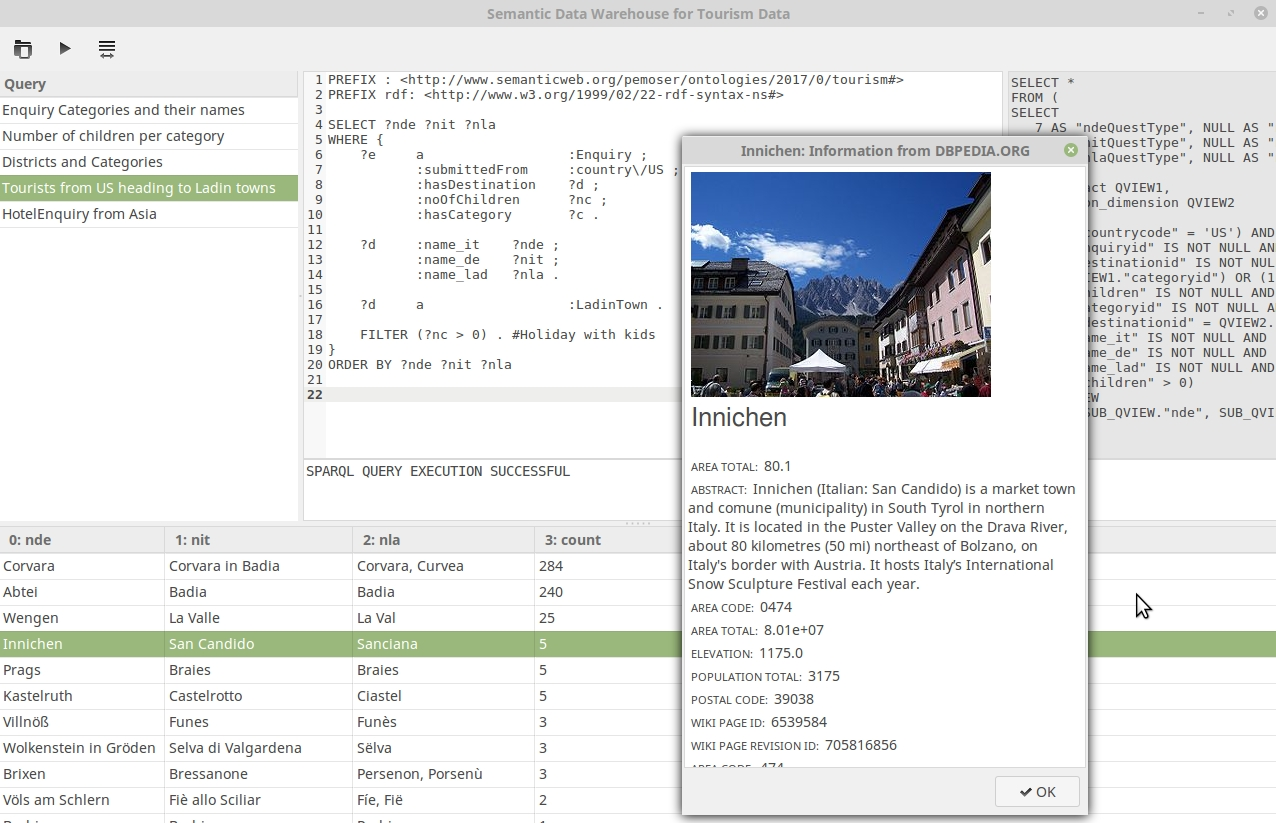
\includegraphics[width=0.7\linewidth]{img/GUI}
\caption{Graphical User Interface of my Semantic Java Application}
\label{fig:GUI}
\end{figure}

\subsection{Used libraries and tools}

In summary I used the following:
\begin{itemize}
\item GTK+ bindings for Java, namely \textit{java-gnome}
\item \textsc{Ontop} framework
\item \textsc{RDF4J} library
\item \textsc{PostgreSQL} as database
\item \textsc{Protege} workbench to generate the OWL and OBDA files
\end{itemize}

I generated the user interface with GTK+ bindings for Java, namely \textsc{java-gnome}, and the GUI builder \textsc{Glade}. Then I searched for the SPARQL query file parser used in the \textsc{Ontop} plugin for \textsc{Protege}, but did not find it immediately. Therefore, I thought to quickly write a preliminary version my self. It parses a \textit{tourism.q} or \textit{dbpedia.q} file, and gives for each \textit{QueryItem} the code section.  Secondly, I reused the \textit{org.semanticweb.ontop.examples.QuestOWLExample} class as a basis to build my own query executor. Third, I wrote an GTK-event-handler to connect to a remote SPARQL repository, and retrieve all literals from a single query. If the \textit{long IRI} toggle is deactivated, I fetch the prefixes from the SPARQL query, and replace each IRI inside the result with its prefix. The following chapter describes how I used \textsc{Quest} and \textsc{RDF4J}.

On the development side, I used \textsc{Eclipse}, \textsc{Maven}, and \textsc{Git}.

\subsection{Applying Semantic Techniques}
In this section I will explain which semantic techniques I used within this project, and how it got implemented in Java. I start with \textsc{Ontop}, \textsc{Quest}, and the \textsc{Owl Api}.

I loaded the \textit{.owl} file and \textit{.obda} file, and created an \textit{OWLOntology}, and a \textit{OBDAModel} from them. Then I had to prepare the configuration for Quest. I reused the code an created a ''Virtual ABox'' mode setup. This means,  that \textsc{Ontop} gets as input a set of mappings (given by the OBDA file), and does just translate the given SPARQL queries over the ontology from the OWL file to SQL queries over the database (in our case PostgreSQL). In contrast, a ''Classic ABox'' mode would need an ontology and data triples to ABOX assertions\footnote{\url{https://github.com/ontop/ontop/wiki/Ontop-Preferences}}. However, the former method is used here.

Then, I generate a quest OWL factory with the previously defined preferences, and obda model, to get a reasoner over this ontology, which can be used to create an statement for \textsc{Quest} out of a given SPARQL query string.

Finally, I retrieved the translated SQL query with \textit{getUnfolding}, and executed the statement with the \textit{executeTuple} method. The result set contained then a signature, that is, all targets from the defined select list of the query (projection), and the bindings to each OWL object, that is, the values of the result.

In addition, I used the \textsc{Rdf4J} framework as follows:
\begin{itemize}
\item Opened connection to \textit{\url{http://dbpedia.org/sparql}} endpoint
\item Executed the query in two steps: First, by preparing a executable statement with \textit{prepareTupleQuery}, and second, by executing it with \textit{evaluate}
\item The result set provides an iterator interface, where I could retrieve all binding sets step-by-step
\item I fetched the thumbnail of each town given by the \textit{thumbnail} value of each retrieved tuple (the redirection of that URL gave some troubles initially, but I could solve that issue by reading the HTTP headers, and issuing a second fetch request.)
\end{itemize}

\subsection{Problem with Semantic Techniques}
I had two problems with the structure of the ontology graph of \textit{dbpedia.org}. On one hand, some information is redundant and therefore multiple instances of the same key/value pair showed up in the results. I have seen that this happened because the IRI was different, but contained the same key finally. For instance, \textit{populationTotal} has two IRIs, namely
\begin{lstlisting}
http://dbpedia.org/property/populationTotal
http://dbpedia.org/ontology/populationTotal
\end{lstlisting}

On the other hand, no unique literal pattern has been defined for city/town names. For example, the town with a German name \textit{Kastelruth} has an Italian correspondence of \textit{Castelrotto,\_South\_Tyrol}. In addition, some predicates are defined for English \textit{dbpedia.org} entries, that do not exist in other \textit{dpbedia.org} versions for other languages. The unique identifier, that I is common in Italy to identify cities or towns is the so-called ISTAT code, from the national statistics Bureau, but there is no such entry in dbpedia. However, I have found a SPARQL endpoint for ISTAT at last, which may be a better endpoint for my needs. Hopefully, I can continue with my project later on to make it really useful.